% Ubah judul dan label berikut sesuai dengan yang diinginkan.
\section{Desain dan Implementasi}
\label{sec:desaindanimplementasi}

\begin{enumerate}[label=\Alph*.]
    \item Diagram Blok Sistem
    \label{subsec:diagrambloksistem}

    \hspace*{1em} Sistem yang telah dirancang memiliki beberapa komponen utama: sensor, kontrol, sistem mekanik, dan motion data. Bagian sensor mencakup load cell di setiap telapak kaki robot untuk mendeteksi beban dan menjaga keseimbangan. Bagian kontrol melibatkan mikrokontroler yang mengolah data sensor dan mengontrol gerakan robot. Sistem mekanik mencakup kerangka robot dengan berbagai servo untuk menggerakkan robot. Bagian motion data menyimpan gerakan yang telah dirancang dalam sistem file mikrokontroler, berisi array target posisi servo dan waktu yang diperlukan untuk mencapainya. Diagram blok sistem robot humanoid dapat dilihat pada Gambar \ref{fig:Diagram_Sistem}.

    \begin{figure} [h] \centering
        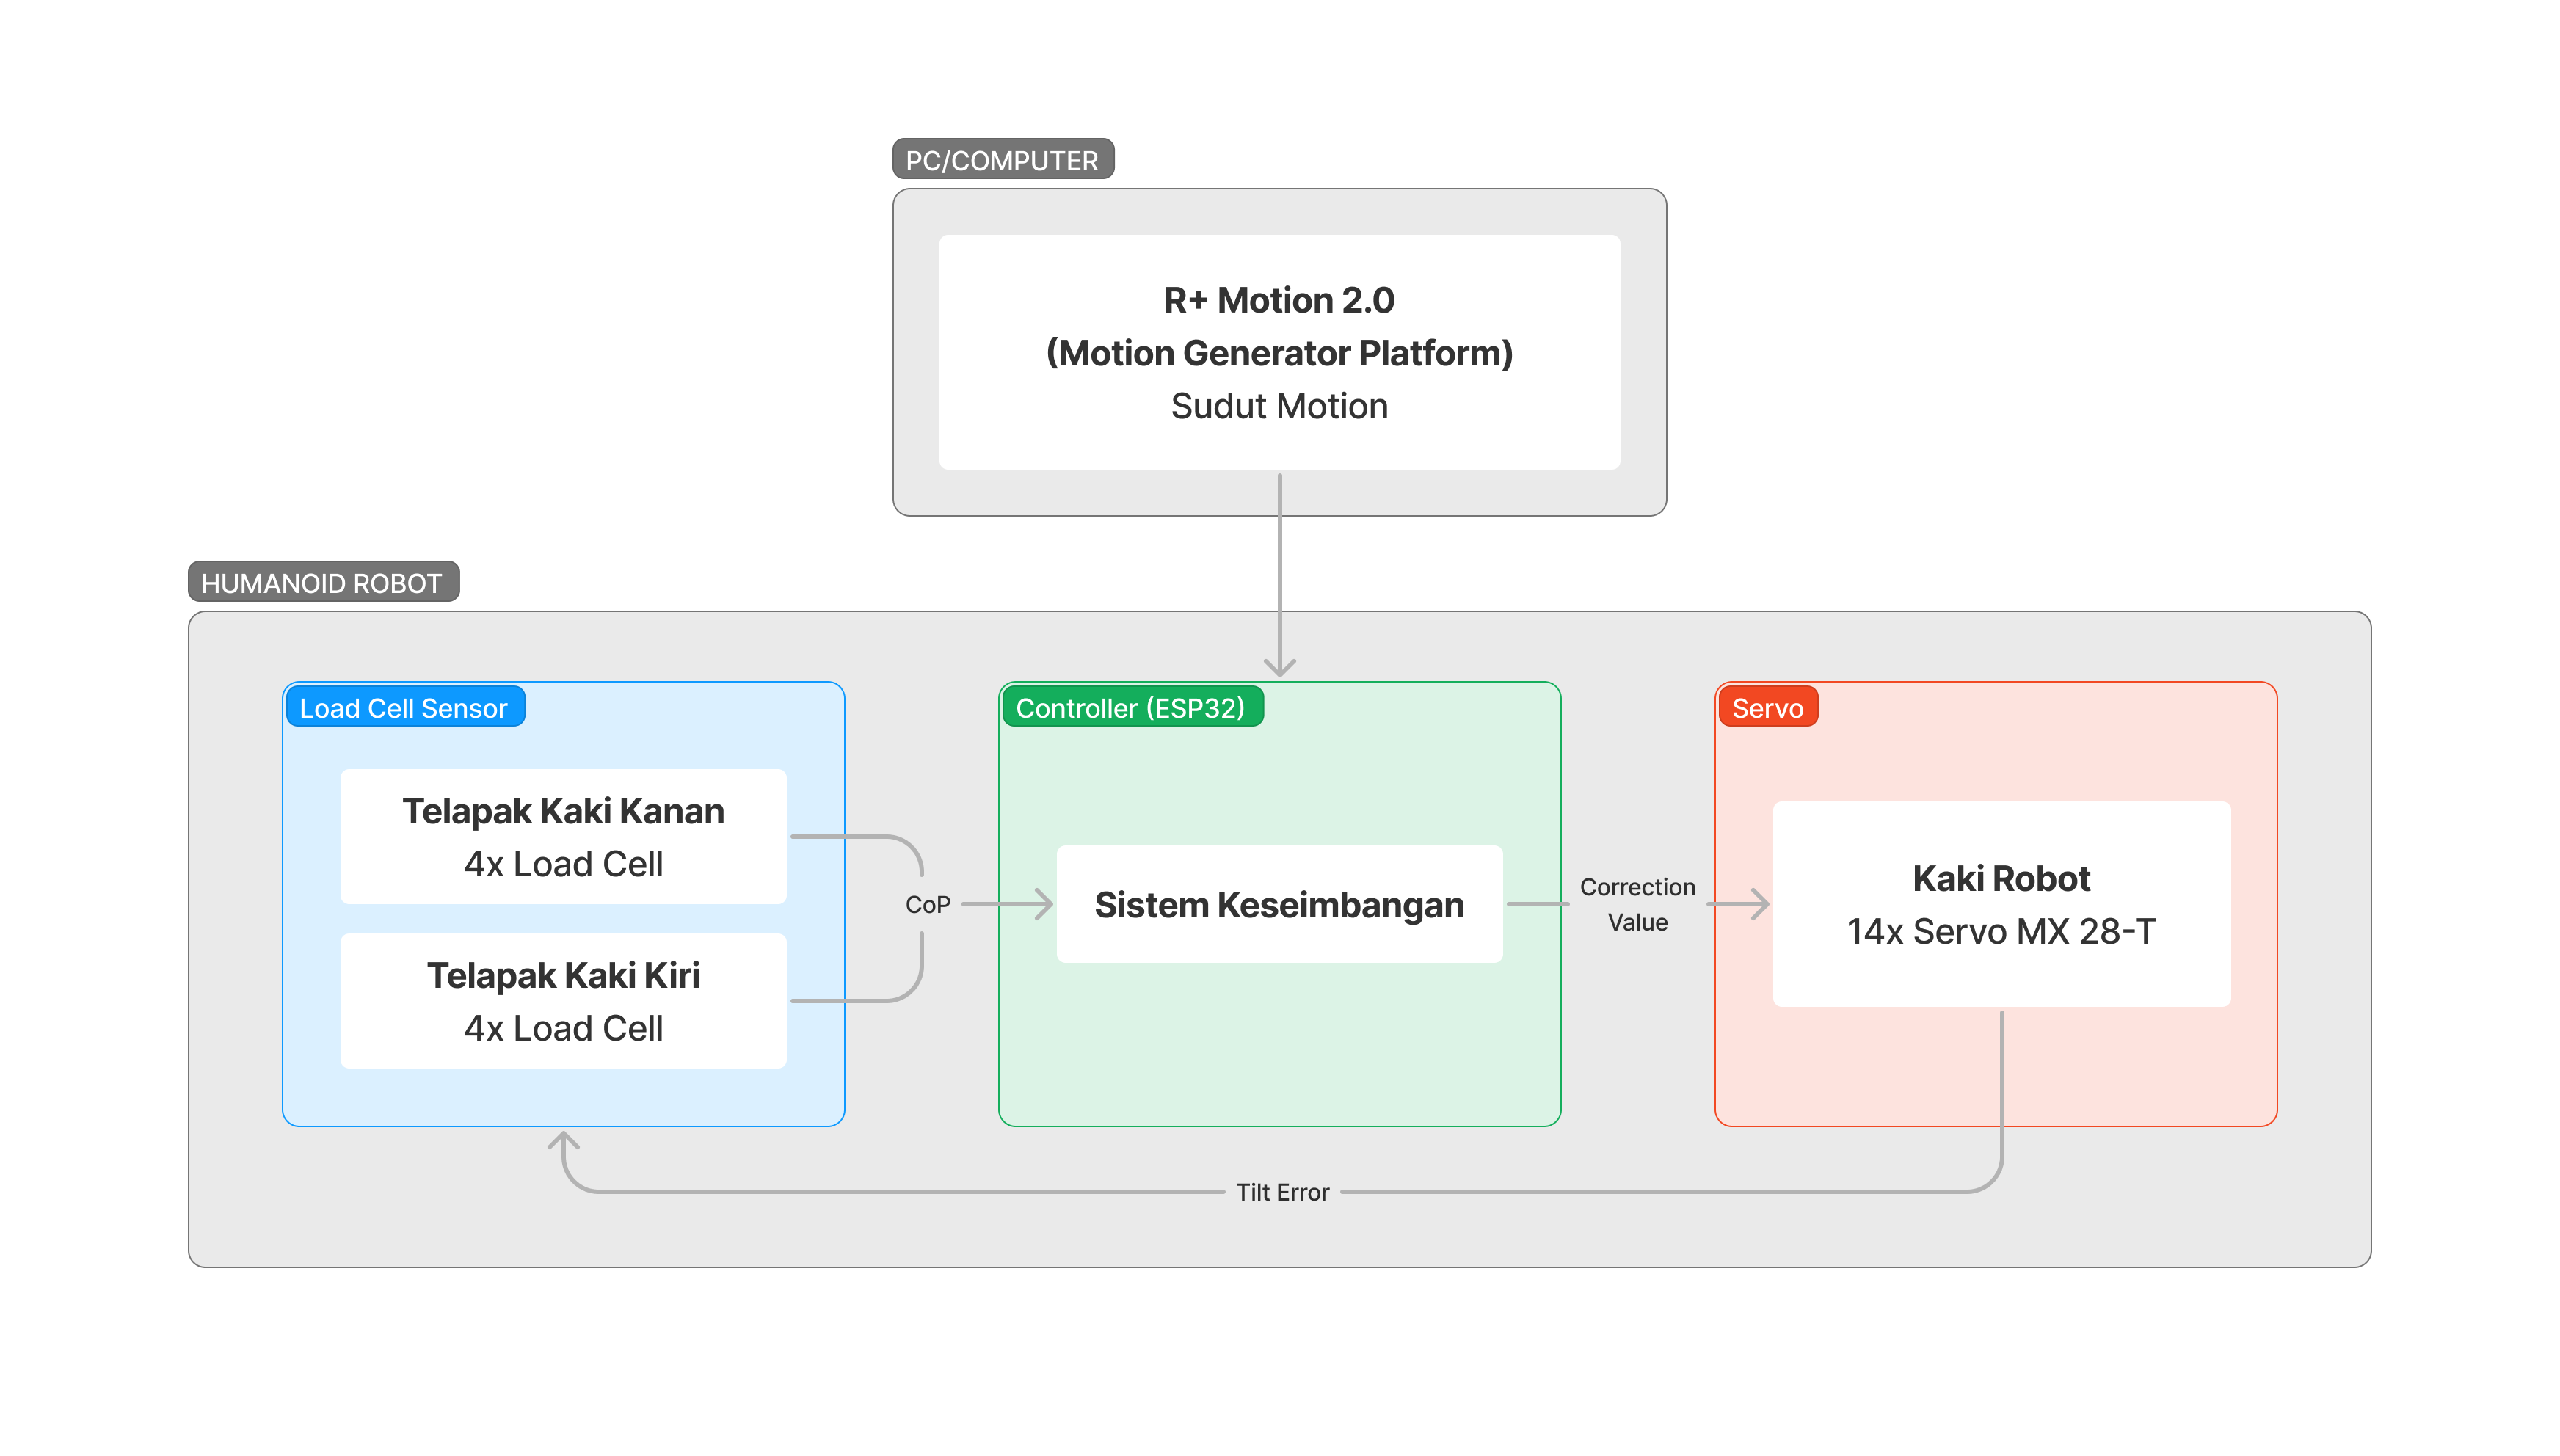
\includegraphics[width=0.45\textwidth]{gambar/Diagram_Sistem.png}
        \caption{Diagran Sistem}
        \label{fig:Diagram_Sistem}
    \end{figure}

    \item Sistem Mekanik
    \label{subsec:sistemmekanik}

    \hspace*{1em} Desain tubuh robot humanoid ini mencakup 29 motor servo. Tubuh bagian atas menggunakan 15 servo tipe XL-320, sedangkan tubuh bagian bawah menggunakan 14 servo tipe MX-28. Rincian desain, ukuran, dan penamaan ID servo pada robot dapat dilihat pada Gambar \ref{fig:Desain_Mekanik}. Informasi tentang derajat kebebasan robot dapat ditemukan pada Tabel \ref{tab:DOF_Robot}, sementara dimensi robot tercantum dalam Tabel \ref{tab:Dimensi_Robot}.

    \begin{figure} [h] \centering
      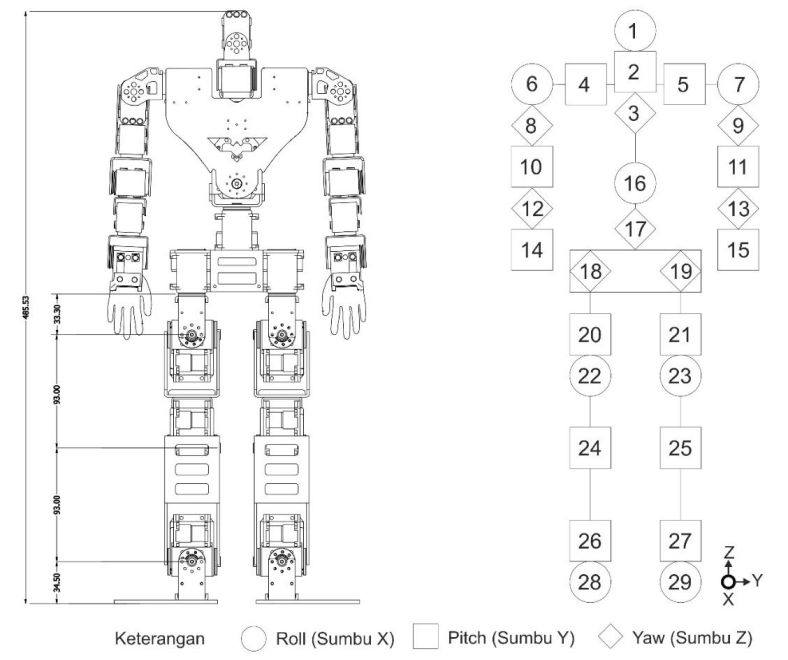
\includegraphics[width=0.35\textwidth]{gambar/Desain_Mekanik.png}
      \caption{Desain Mekanik Robot}
      \label{fig:Desain_Mekanik}
    \end{figure}

    % Tabel untuk Degree of Freedom (DOF)
    \begin{table}[htb]
      \centering
      \caption{Derajat Kebebasan (DOF) dari Body Part}
      \begin{tabular}{>{\itshape}l >{\itshape}l >{\itshape}l}
        \toprule
        \textit{Body Part} & \textit{DOF} & \textit{Total} \\
        \midrule
        Head & 3 DOF & 3 \\
        Arm (Shoulder) & 2 DOF x 2 & 4 \\
        Arm (Elbow) & 2 DOF x 2 & 4 \\
        Arm (Hand/Wrist) & 2 DOF x 2 & 4 \\
        Torso & 2 DOF & 2 \\
        Leg (Hip) & 3 DOF x 2 & 6 \\
        Leg (Knee) & 1 DOF x 2 & 2 \\
        Leg (Ankle) & 2 DOF x 2 & 4 \\
        \midrule
        Total & & 29 \\
        \bottomrule
      \end{tabular}
      \label{tab:DOF_Robot}
    \end{table}

    % Tabel dengan Teks Italic
    \begin{table}[h]
      \centering
      \caption{Dimensi Robot}
      \begin{tabular}{>{\itshape}l >{\itshape}l}
        \toprule
        \textit{Dimension} & \textit{Length (mm)} \\
        \midrule
        Height & 485 \\
        Width (Shoulder to Shoulder) & 116 \\
        Depth (Chest to Back) & 45 \\
        Length of Upper Leg & 124.5 \\
        Length of Lower Leg & 127.5 \\
        Length between hip joints & 73.8 \\
        Length of Upper Arm & 97 \\
        Length of Lower Arm & 128.5 \\
        Width of sole & 84.5 \\
        Length of sole & 135.5 \\
        \bottomrule
      \end{tabular}
      \label{tab:Dimensi_Robot}
    \end{table}

    \item Sistem Elektronik
    \label{subsec:sistemelektronik}

    \hspace*{1em} Sistem perangkat keras (hardware) dalam penelitian ini dijelaskan melalui diagram blok yang ditunjukkan pada Gambar \ref{fig:Diagram_Elektronik}. Sistem ini menggunakan sistem tertanam yang terdiri dari mikrokontroler ESP32 dan ESP32-C3. Sistem tertanam dipilih karena robot yang dikembangkan dalam penelitian ini merupakan pengembangan dari penelitian sebelumnya yang dilakukan oleh Fahd (2018). 

    \begin{figure} [h] \centering
      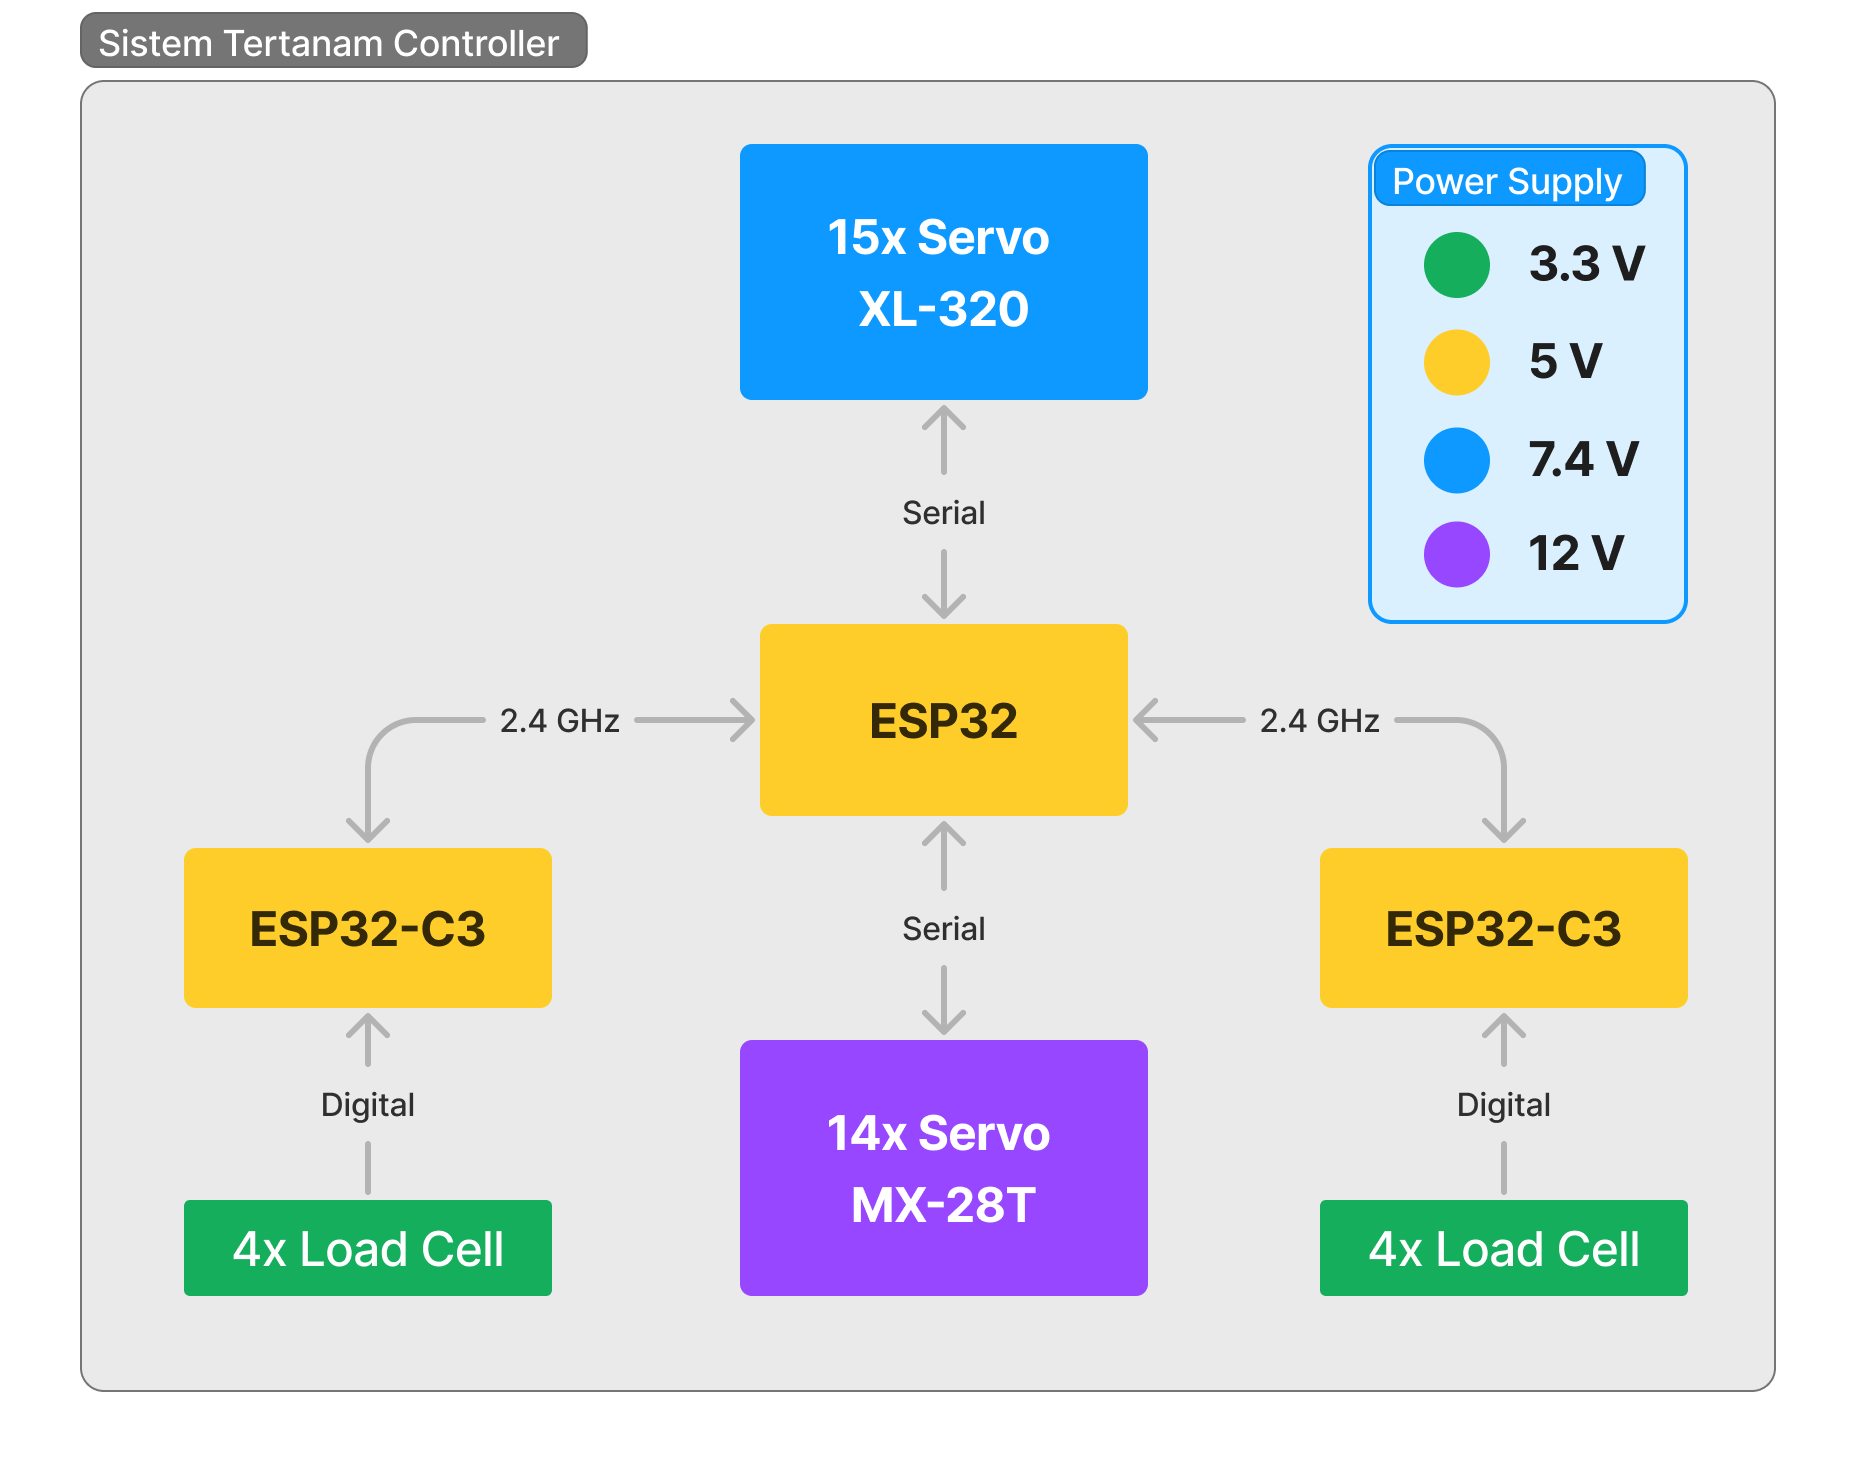
\includegraphics[width=0.4\textwidth]{gambar/Diagram_Elektronik.png}
      \caption{Diagran Elektronik Robot}
      \label{fig:Diagram_Elektronik}
    \end{figure}

    \hspace*{1em} ESP32-C3, digunakan untuk pengambilan data dari load cell dan mengirimkannya ke ESP32. ESP32-C3 memiliki kemampuan Wi-Fi yang sama dengan ESP32, sehingga memungkinkan komunikasi nirkabel antara dua mikrokontroler. ESP32-C3 juga memiliki dimensi yang lebih kecil, sehingga lebih mudah ditempatkan pada kaki robot. 

    \item Desain Sistem Load Cell
    \label{subsec:desainsistemloadcell}

    \hspace*{1em} Setiap telapak kaki robot dilengkapi dengan 4 load cell yang terpasang di ujung-ujung kaki. Masing-masing load cell mendeteksi tekanan, sehingga memungkinkan sistem untuk menentukan posisi pusat tekanan pada telapak kaki robot. Desain telapak kaki robot dapat dilihat pada Gambar \ref{fig:Dia_LoadCell}.
    
    \begin{figure} [h] \centering
      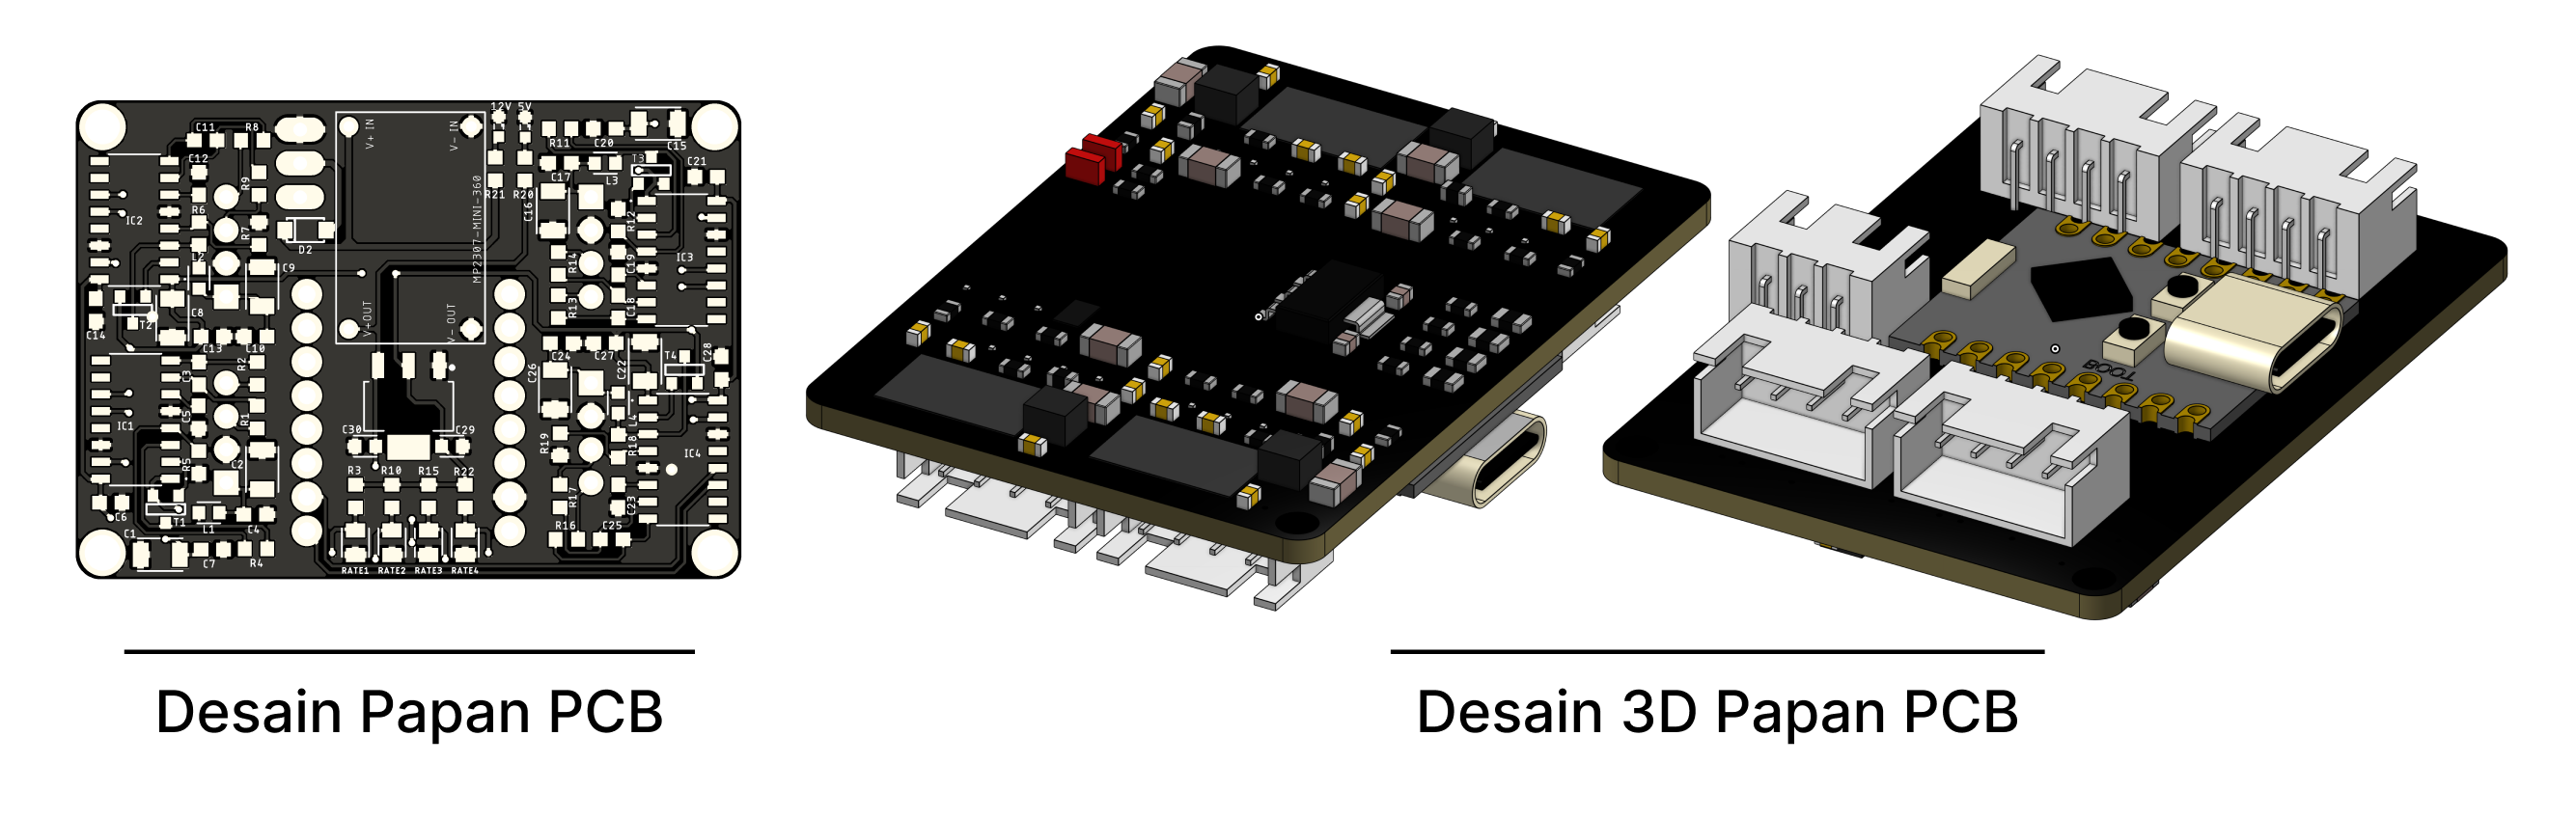
\includegraphics[width=0.4\textwidth]{gambar/Desain_PCB.png}
      \caption{Desain Papan PCB}
      \label{fig:Desain_PCB}
    \end{figure}

    \begin{figure} [h] \centering
        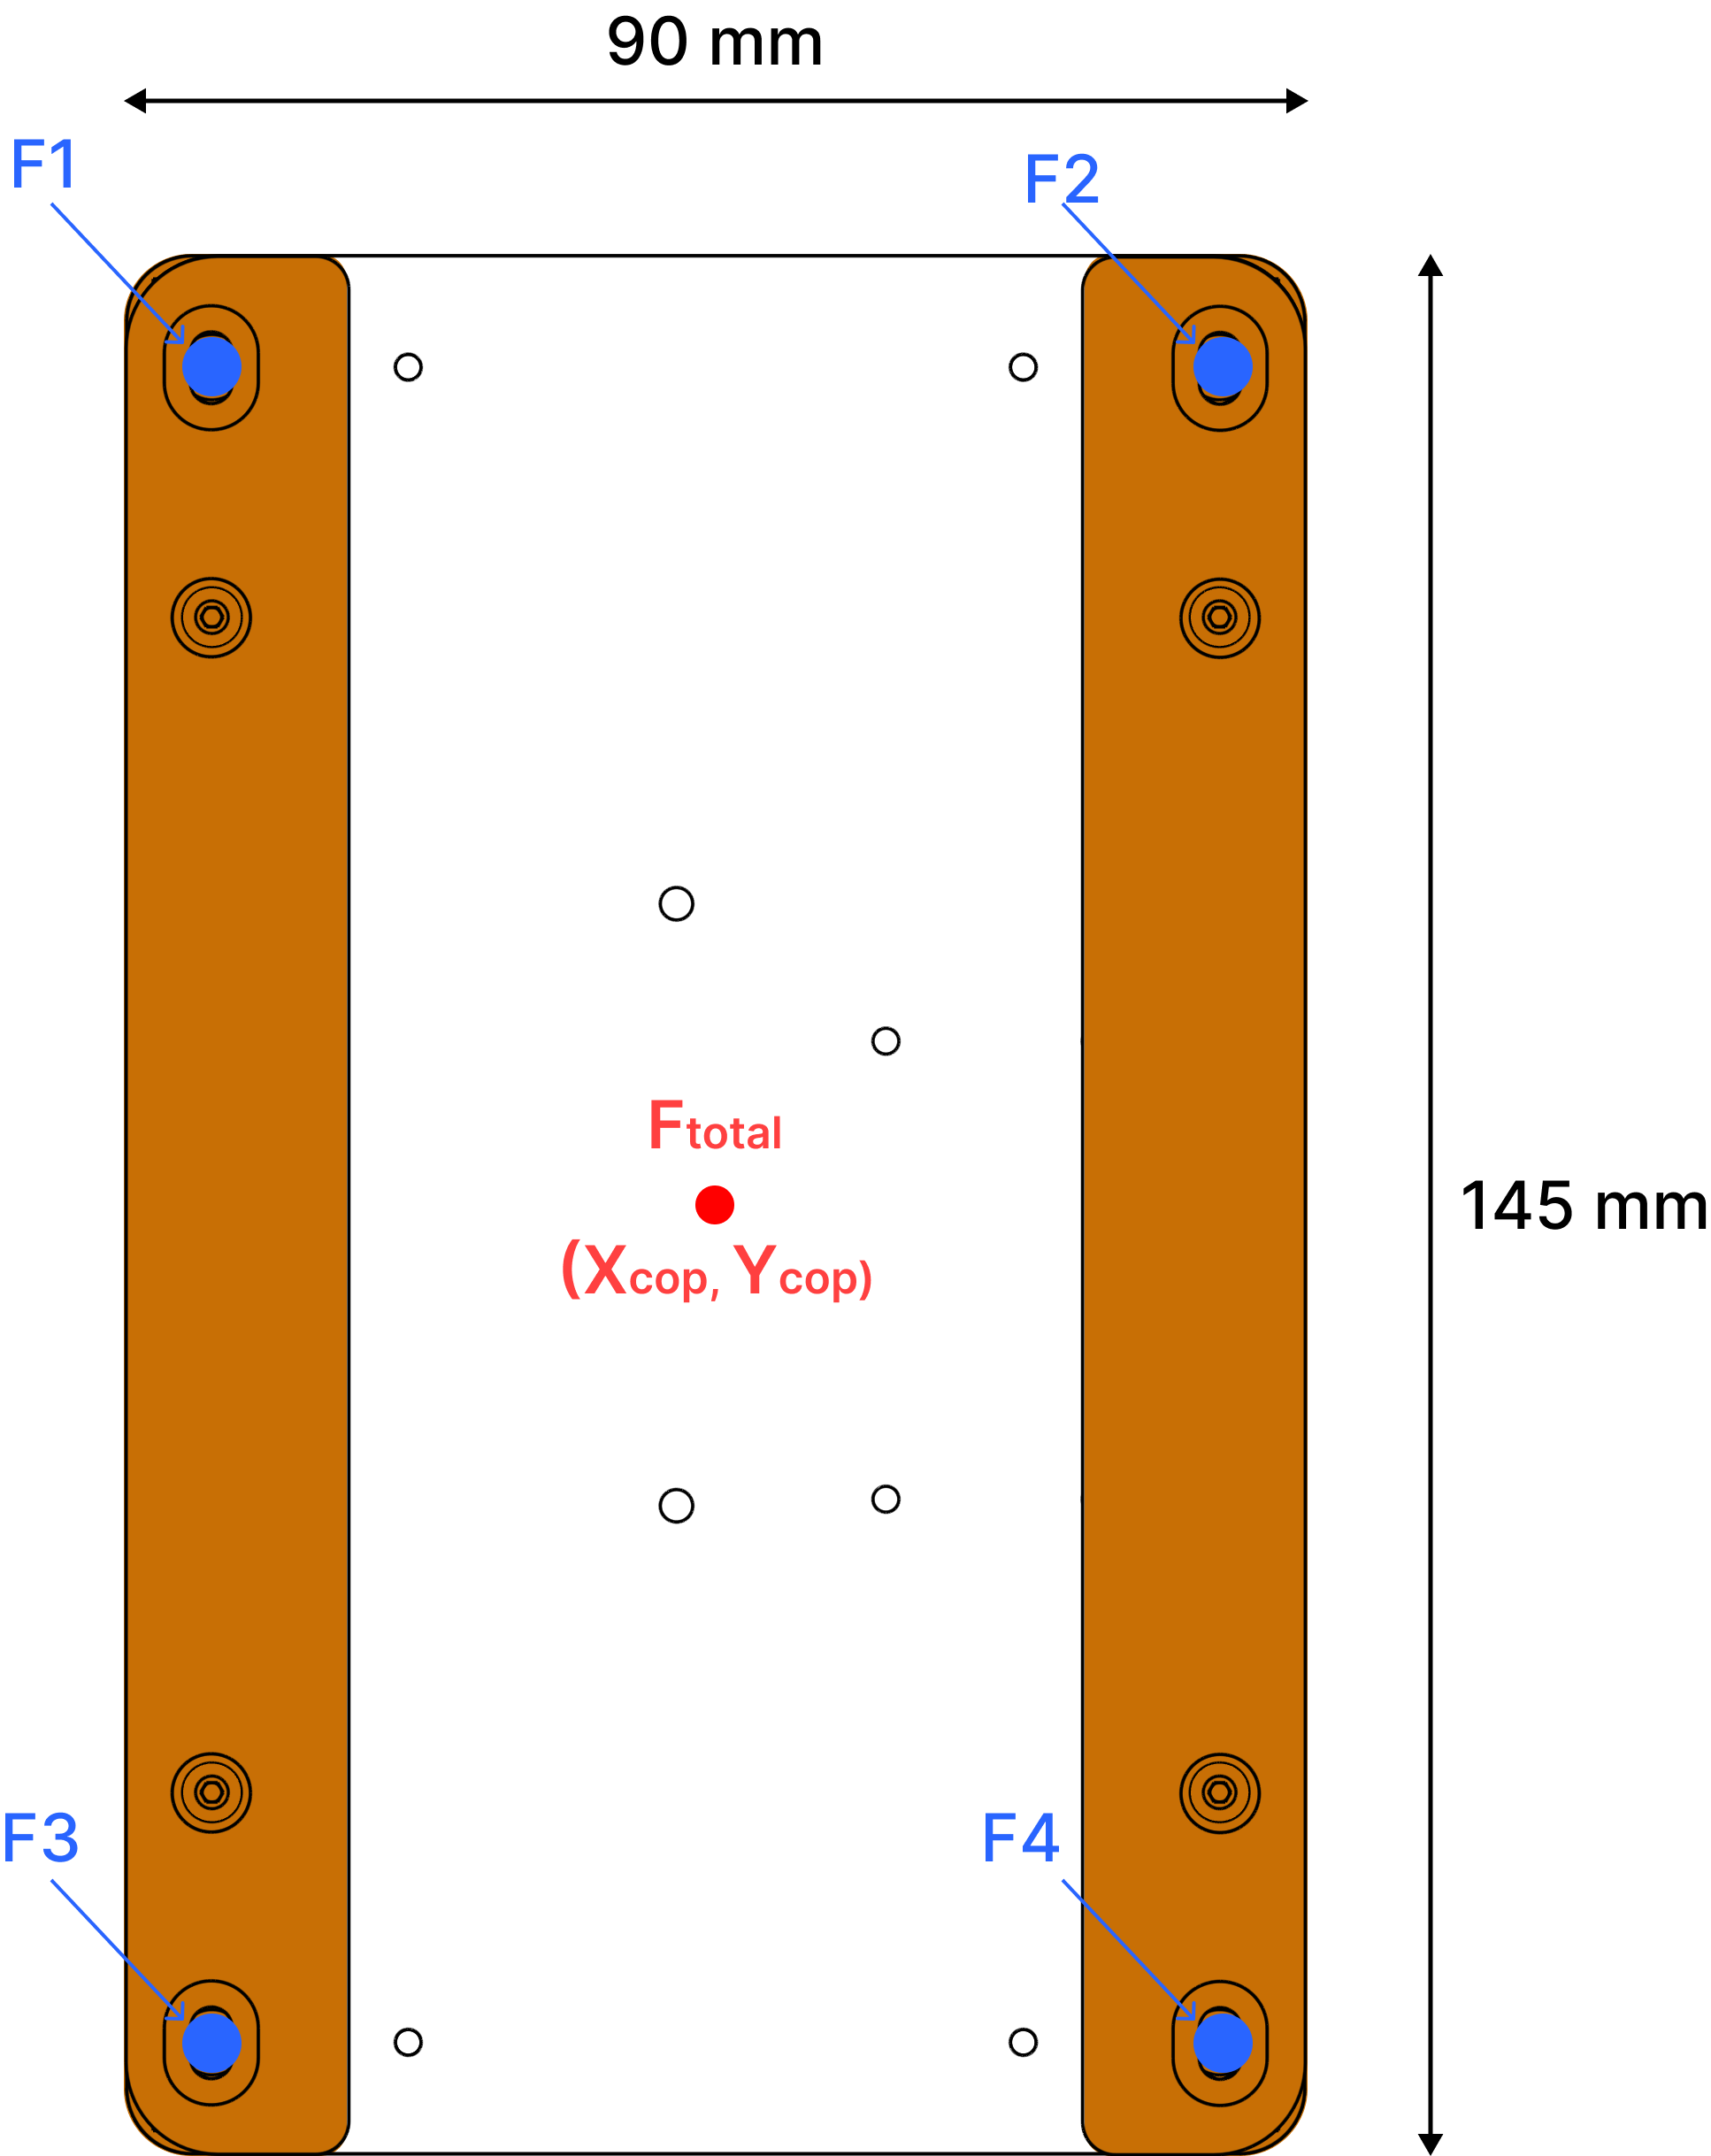
\includegraphics[width=0.3\textwidth]{gambar/Diagram_LoadCell.png}
        \caption{Desain Load Cell pada Telapak Kaki Robot}
        \label{fig:Dia_LoadCell}
    \end{figure}

    \hspace*{1em} Gambar \ref{fig:Desain_PCB} menunjukkan desain jalur PCB yang akan digunakan pada robot. PCB ini memiliki dimensi 50 x 36 mm dengan dua lapisan (layer). Lapisan atas berisi komponen SMD, sementara lapisan bawah mencakup konektor dan mikrokontroler. Desain dua lapisan ini memungkinkan penggunaan ruang yang lebih efisien dan memberikan fleksibilitas dalam penempatan komponen.  
    
    \item Pengolahan Data Load Cell
    \label{subsec:firmwaremikrokontroler}

    \hspace*{1em} IC HX711 tidak memiliki internal register, dan komunikasi dengannya dilakukan secara sinkron menggunakan dua pin: pin data (DOUT) dan pin clock (PD\_SCK). Ketika data siap diambil, pin data berubah menjadi logika rendah. Untuk mengambil data, kita perlu mengirim 25 hingga 27 pulsa ke pin clock, dengan 25 pulsa untuk penguatan (gain) 128. Jika pin data berubah menjadi logika tinggi, data sudah siap diambil; jika tetap rendah, data belum siap. Untuk menghindari blocking saat membaca data dari beberapa \emph{load cell}, dapat digunakan pendekatan konkurensial seperti pada Gambar \ref{fig:Task_LoadCell}.

    \begin{figure} [h] \centering
      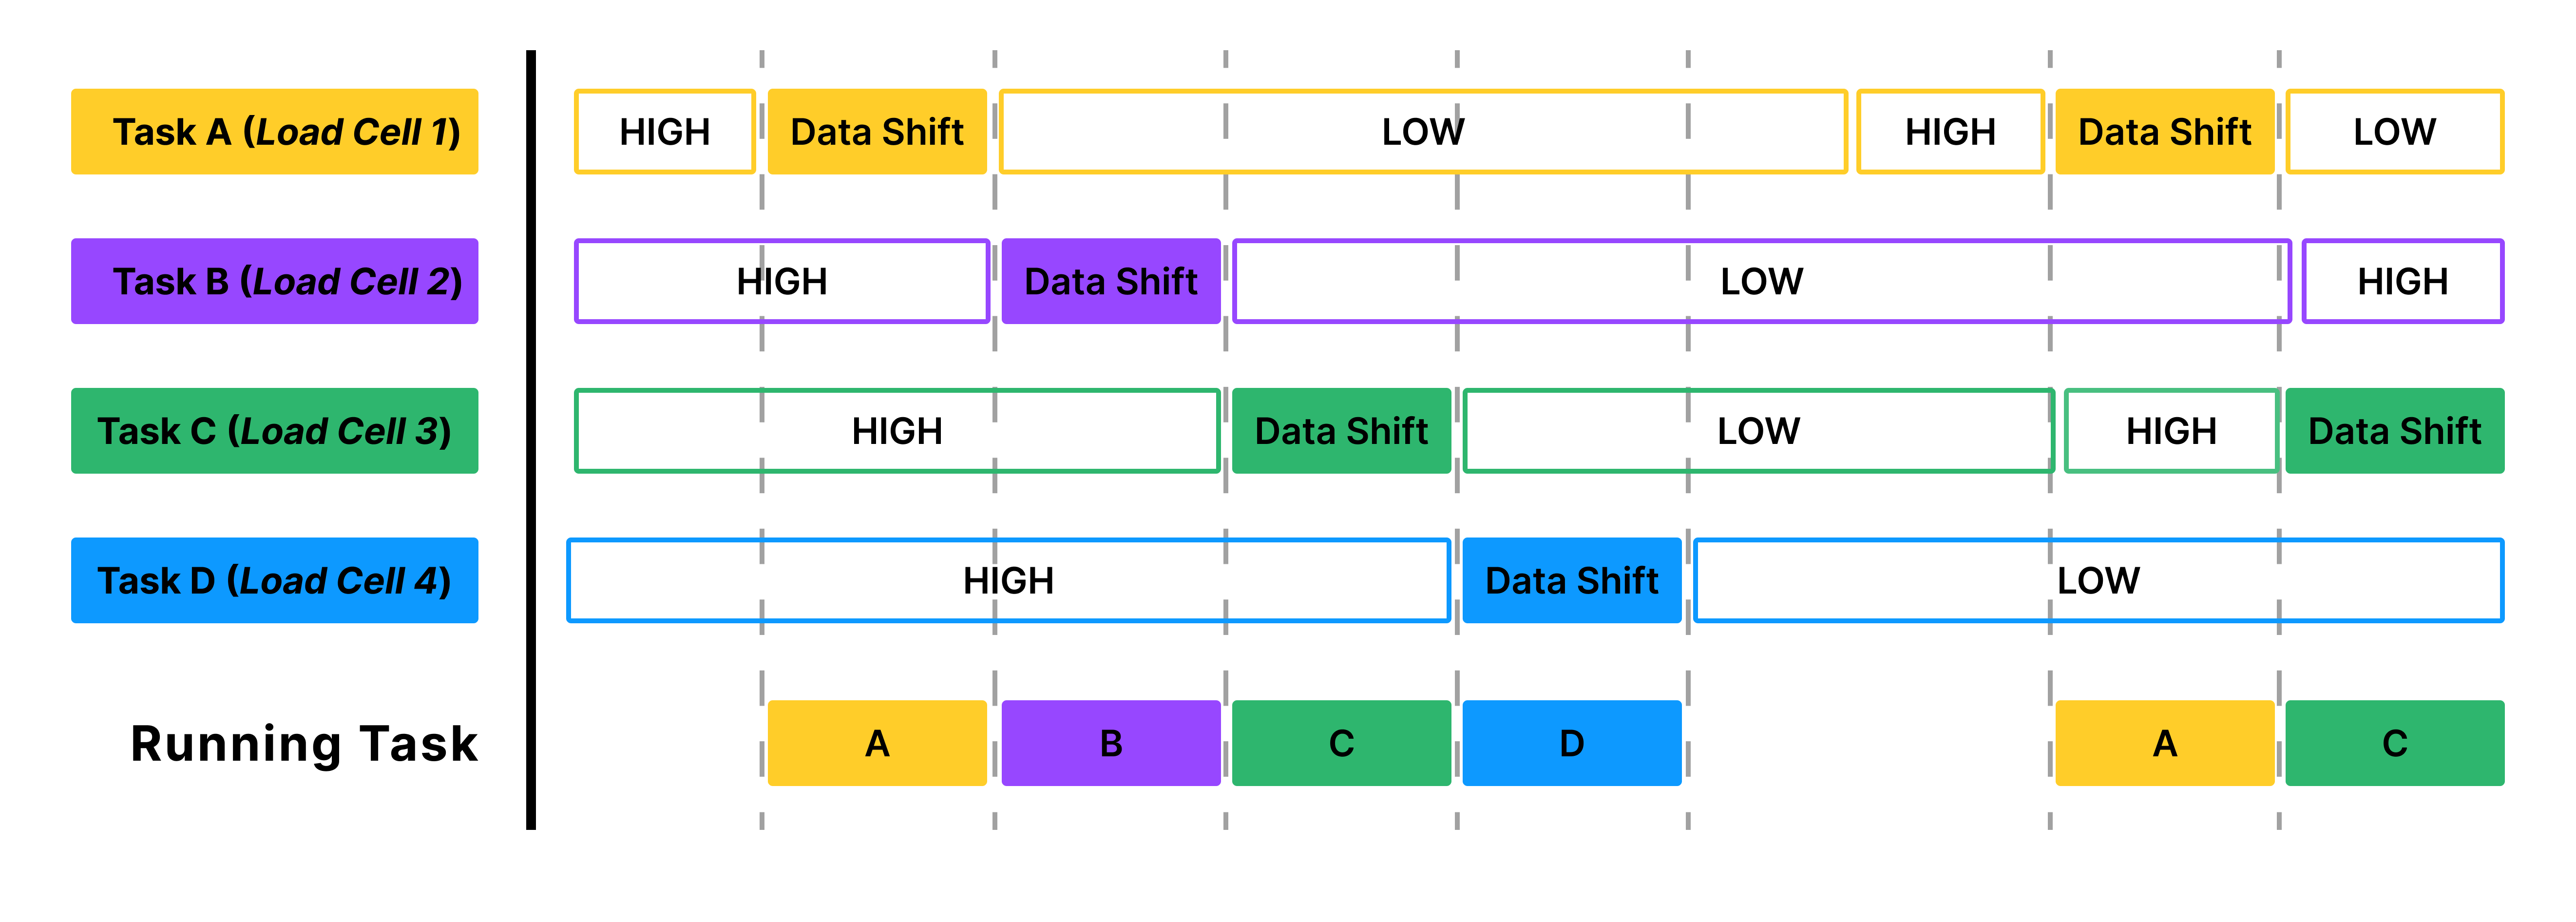
\includegraphics[width=0.4\textwidth]{gambar/Task_LoadCell.png}
      \caption{Concurrent Task pada Pembacaan \emph{Load Cell}}
      \label{fig:Task_LoadCell}
    \end{figure}

    \hspace*{1em} ESP32 menggunakan FreeRTOS yang mendukung multitasking, memungkinkan beberapa tugas berjalan bersamaan. Dalam contoh ini, empat tugas masing-masing bertanggung jawab membaca data dari empat \emph{load cell} yang berbeda. Setiap tugas mengirimkan pulsa ke pin clock dan membaca data dari pin data. Setelah satu tugas selesai, tugas berikutnya dapat membaca data dari \emph{load cell} lain. Pendekatan ini memungkinkan pembacaan data dari berbagai \emph{load cell} tanpa menghambat tugas lainnya, meningkatkan efisiensi dan kinerja sistem.


    \item Algoritma Program Pemanggilan \textit{Motion}
    \label{subsec:algoritmamotion}

    \hspace*{1em} Sebelum robot dijalankan, program yang juga berisi data motion yang sudah dibuat sebelumnya diunggah ke dalam memori non-volatile pada  mikrokontroler. Motion yang diunggah berisi data untuk servo motor bagian atas dan bawah robot. Selanjutnya, robot dijalankan dan dimasukan input berupa index motion. Tiap index motion memiliki beberapa frame berdasarkan data motion yang telah diupload. Kemudian robot akan menjalankan gerakan satu persatu berdasarkan frame dari index motion yang dimasukkan.

    \begin{figure} [h]
      \centering
      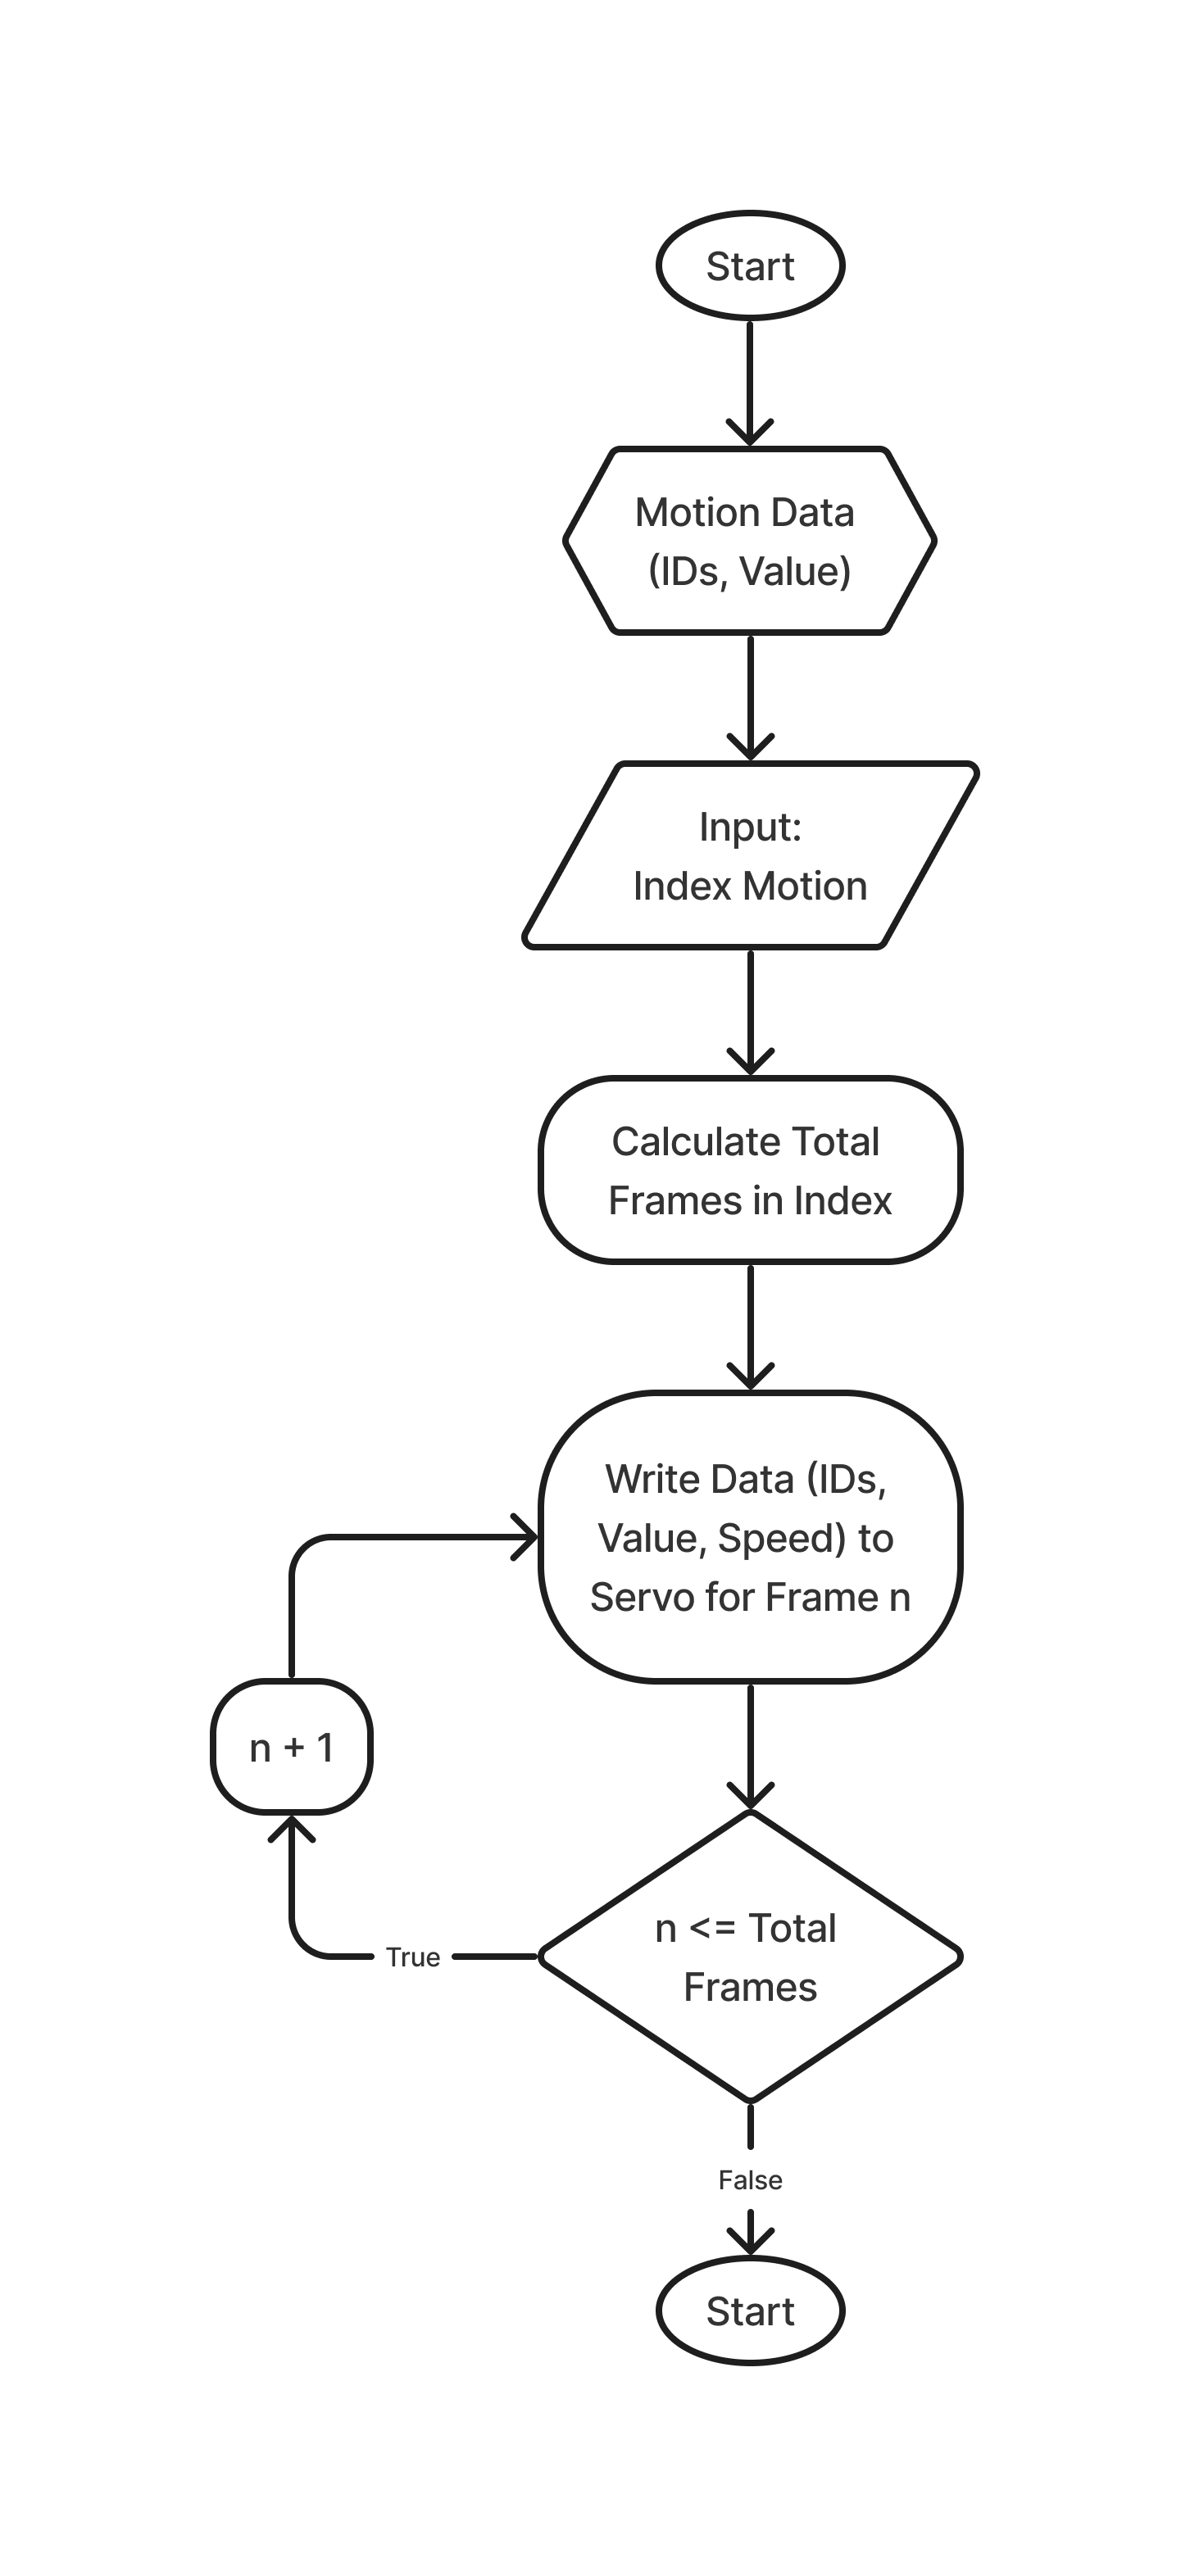
\includegraphics[width=0.3\textwidth]{gambar/flowchart_play_index.png}
      \caption{Diagram Alir Program Berjalan}
      \label{fig:Algoritma_Berjalan}
    \end{figure}

    \item Perhitungan Pusat Tekanan terhadap Robot
    \label{subsec:perhitunganpusattekanan}

    \hspace*{1em} Tekanan pada masing-masing load cell dijumlah dengan persamaan \ref{eq:Total_Force}. Hasil dari penjumlahan tersebut kemudian digunakan untuk menghitung posisi pusat tekanan pada sumbu x dan y dengan persamaan \ref{eq:COP_X} dan \ref{eq:COP_Y}. Pada posisi seimbang, posisi pusat tekanan akan berada pada titik (0,0) yang berada di tengah-tengah telapak kaki. Pusat tekanan tersebut dihitung dengan menjumlahkan tekanan terhadap titik pusat tekanan pada telapak kaki robot. Rentang nilai pusat tekanan pada telapak kaki robot adalah -1 hingga 1. Hasil dari perhitungan pusat tekanan tersebut kemudian dikirimkan ke mikrokontroler utama yang akan mengontrol gerakan robot. 

    \begin{equation}
      F_{\mathrm{total}} = F_1 + F_2 + F_3 + F_4
      \label{eq:Total_Force}
    \end{equation}

    \begin{equation}
      X_{\mathrm{cop}} = \frac{- F_1 + F_2 - F_3 + F_4}{F_{\mathrm{total}}}
      \label{eq:COP_X}
    \end{equation}

    \begin{equation}
      Y_{\mathrm{cop}} = \frac{F_1 + F_2 - F_3 - F_4}{F_{\mathrm{total}}}
      \label{eq:COP_Y}
    \end{equation}

    \item Algoritma Kontrol PID
    \label{subsec:algoritmakontrolpid}

    \hspace*{1em} Pada penelitian ini, terdapat dua kontrol PID yang digunakan, yaitu kontrol PID Pitch dan kontrol PID Roll. Pada kontrol PID Pitch, input berupa nilai posisi pusat tekanan pada sumbu Y. Sedangkan pada kontrol PID Roll, input berupa nilai posisi pusat tekanan pada sumbu X. Untuk setpoint kontrol PID Pitch dan Roll, digunakan nilai yang sudah ditemukan pada pengambilan data input pusat tekanan sebelumnya. Nilai error diperoleh dari selisih antara posisi pusat tekanan saat ini dengan setpoint seperti pada Persamaan \ref{eq:Error_PID} dan koreksi PID dihitung dengan Persamaan \ref{eq:Koreksi_PID}.

    \begin{equation}
      \mathrm{e} = COP_{\mathrm{error}} = COP_{\mathrm{set}} - COP_{\mathrm{input}}
      \label{eq:Error_PID}
    \end{equation}

    \begin{equation}
      \mathrm{Koreksi} = \mathrm{Kp} \cdot \mathrm{e} + \mathrm{Ki} \cdot \int \mathrm{e} + \mathrm{Kd} \cdot \frac{\mathrm{de}}{\mathrm{dt}}
      \label{eq:Koreksi_PID}
    \end{equation}

    \item Servo Settings as Compensation
    \label{subsec:servosettings}

    \hspace*{1em} The servos used are located at the \textit{hip adduction} and \textit{ankle} because these two parts have a significant impact on the robot's posture stability when standing on one leg. The hip servo functions to control the upper part of the robot, while the ankle servo controls the movement of the foot. By precisely adjusting the servo angles, the robot can make the necessary adjustments to maintain balance when moving or standing on uneven surfaces.

    \begin{figure} [h] \centering
      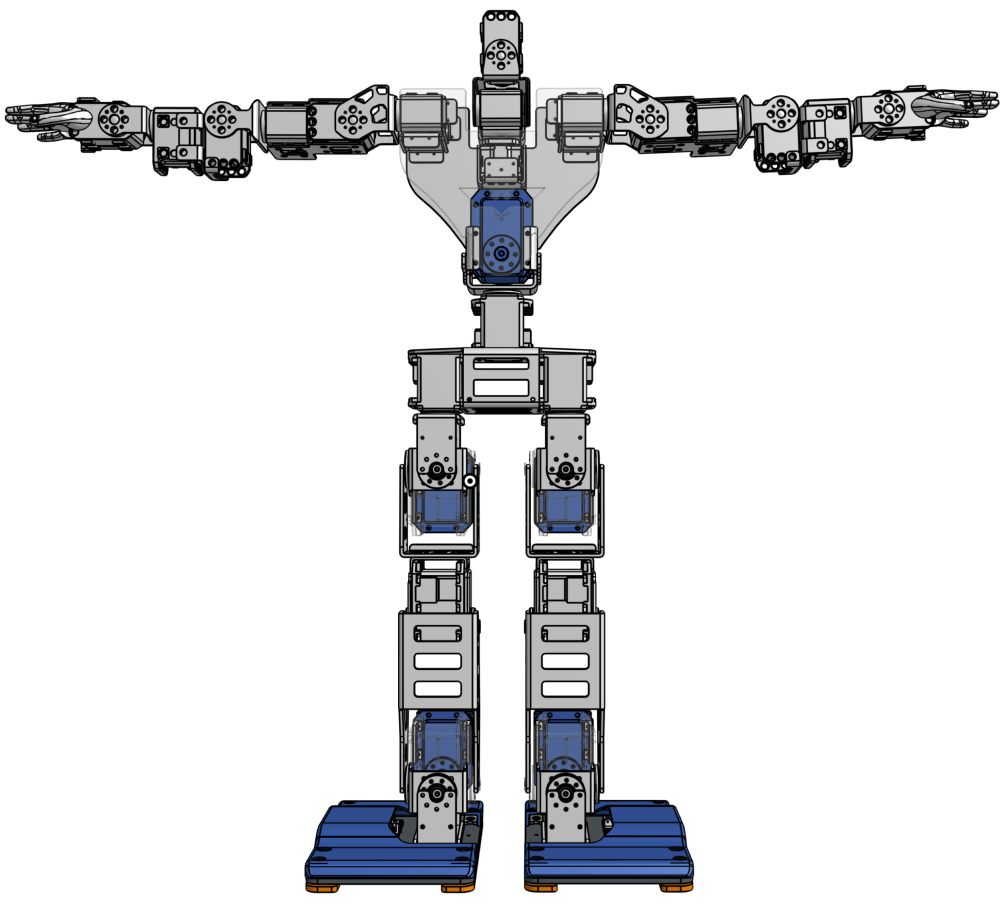
\includegraphics[width=0.4\textwidth]{gambar/controlled_servo.png}
      \caption{Servo Settings as Compensation}
      \label{fig:Controlled_Servo}
    \end{figure}

    \hspace*{1em} In this research, five servos are used to control the roll movement, consisting of two servos on each ankle, one servo on the torso, and two servos on each hip adduction. The servo settings as compensation can be seen in Figure \ref{fig:Controlled_Servo}, indicated by the blue-colored servos.
\end{enumerate}